\section{Experimental evaluation}
\label{Sec:experimental-eval}

Here we report all the test executed to compare the performance between the sequential and parallel version of the A-Star implementation.
All the test are performed on a Linux environment.

\subsection{performance}

\subsubsection{Grid Milan}
The graph generated from the grid of Milan (1024x1024) has around 800k nodes and has random generated weights to increase the difficulty to find the path with the best cost.

\begin{figure}
    \centering
    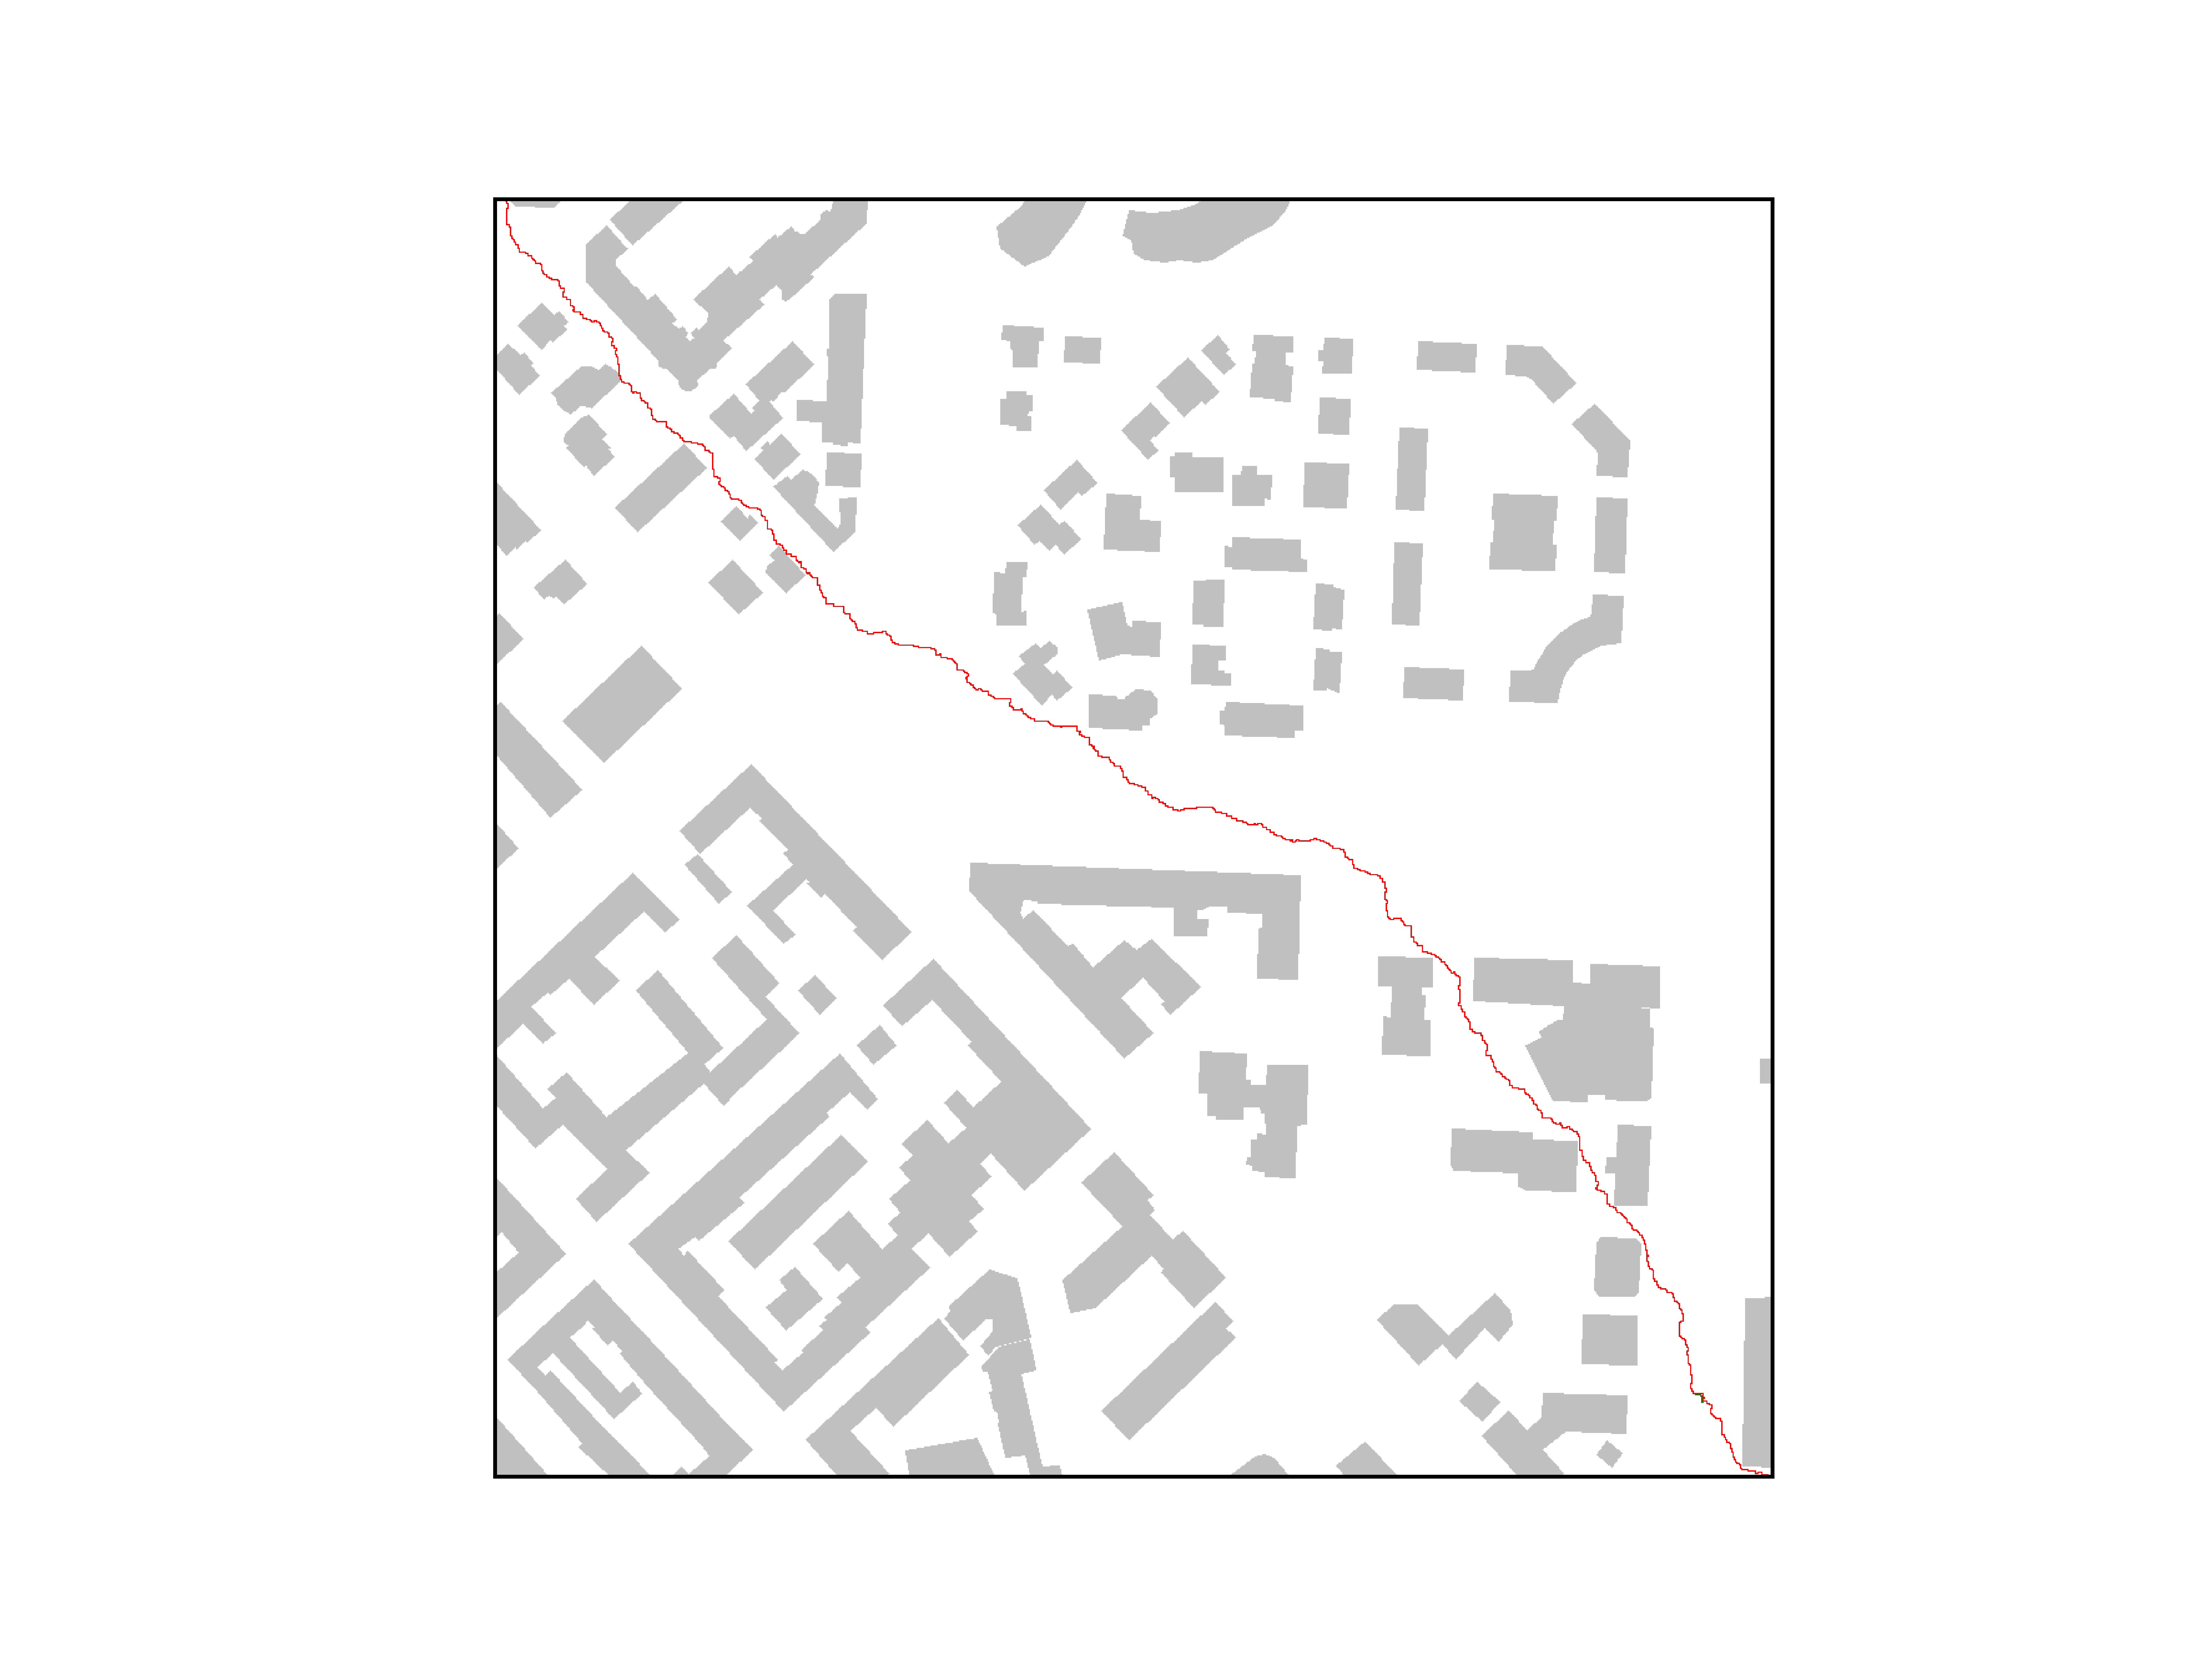
\includegraphics[scale=0.7]{../assets/gridMilan.png}
    \caption{Milan map with path found}
    \label{Milan grid}
\end{figure}

\begin{figure}
    \centering
    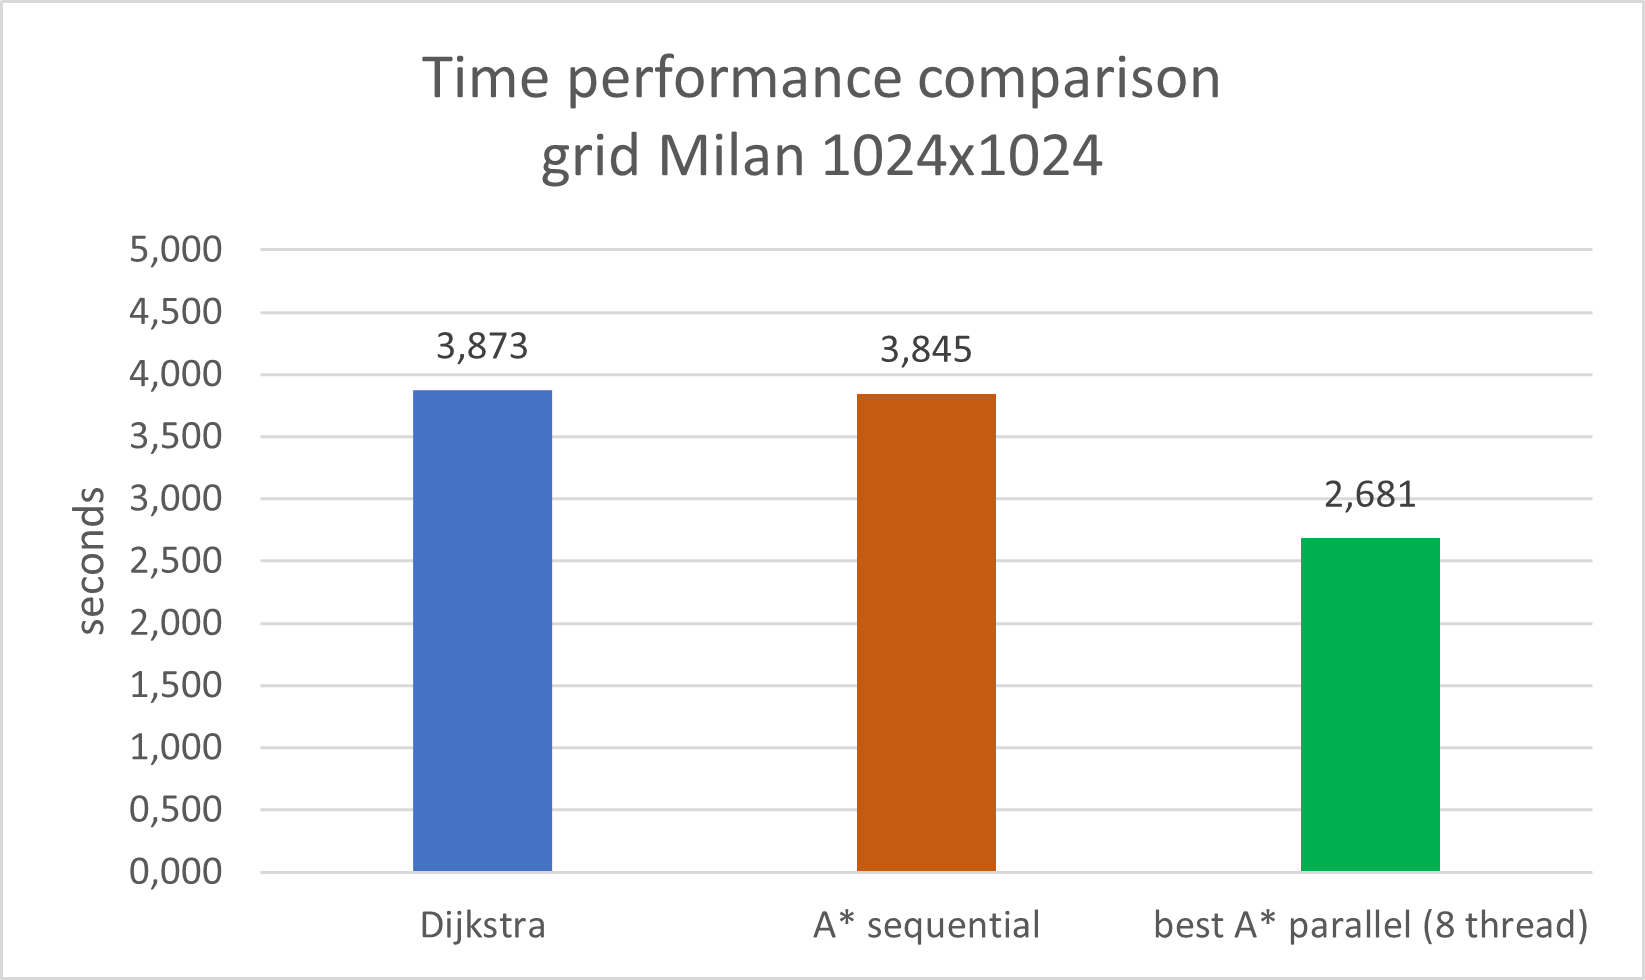
\includegraphics[scale=0.7]{../assets/milanComparison.png}
    \caption{Performance comparison on different algorithms}
    \label{Milan comp}
\end{figure}

\begin{figure}
    \centering
    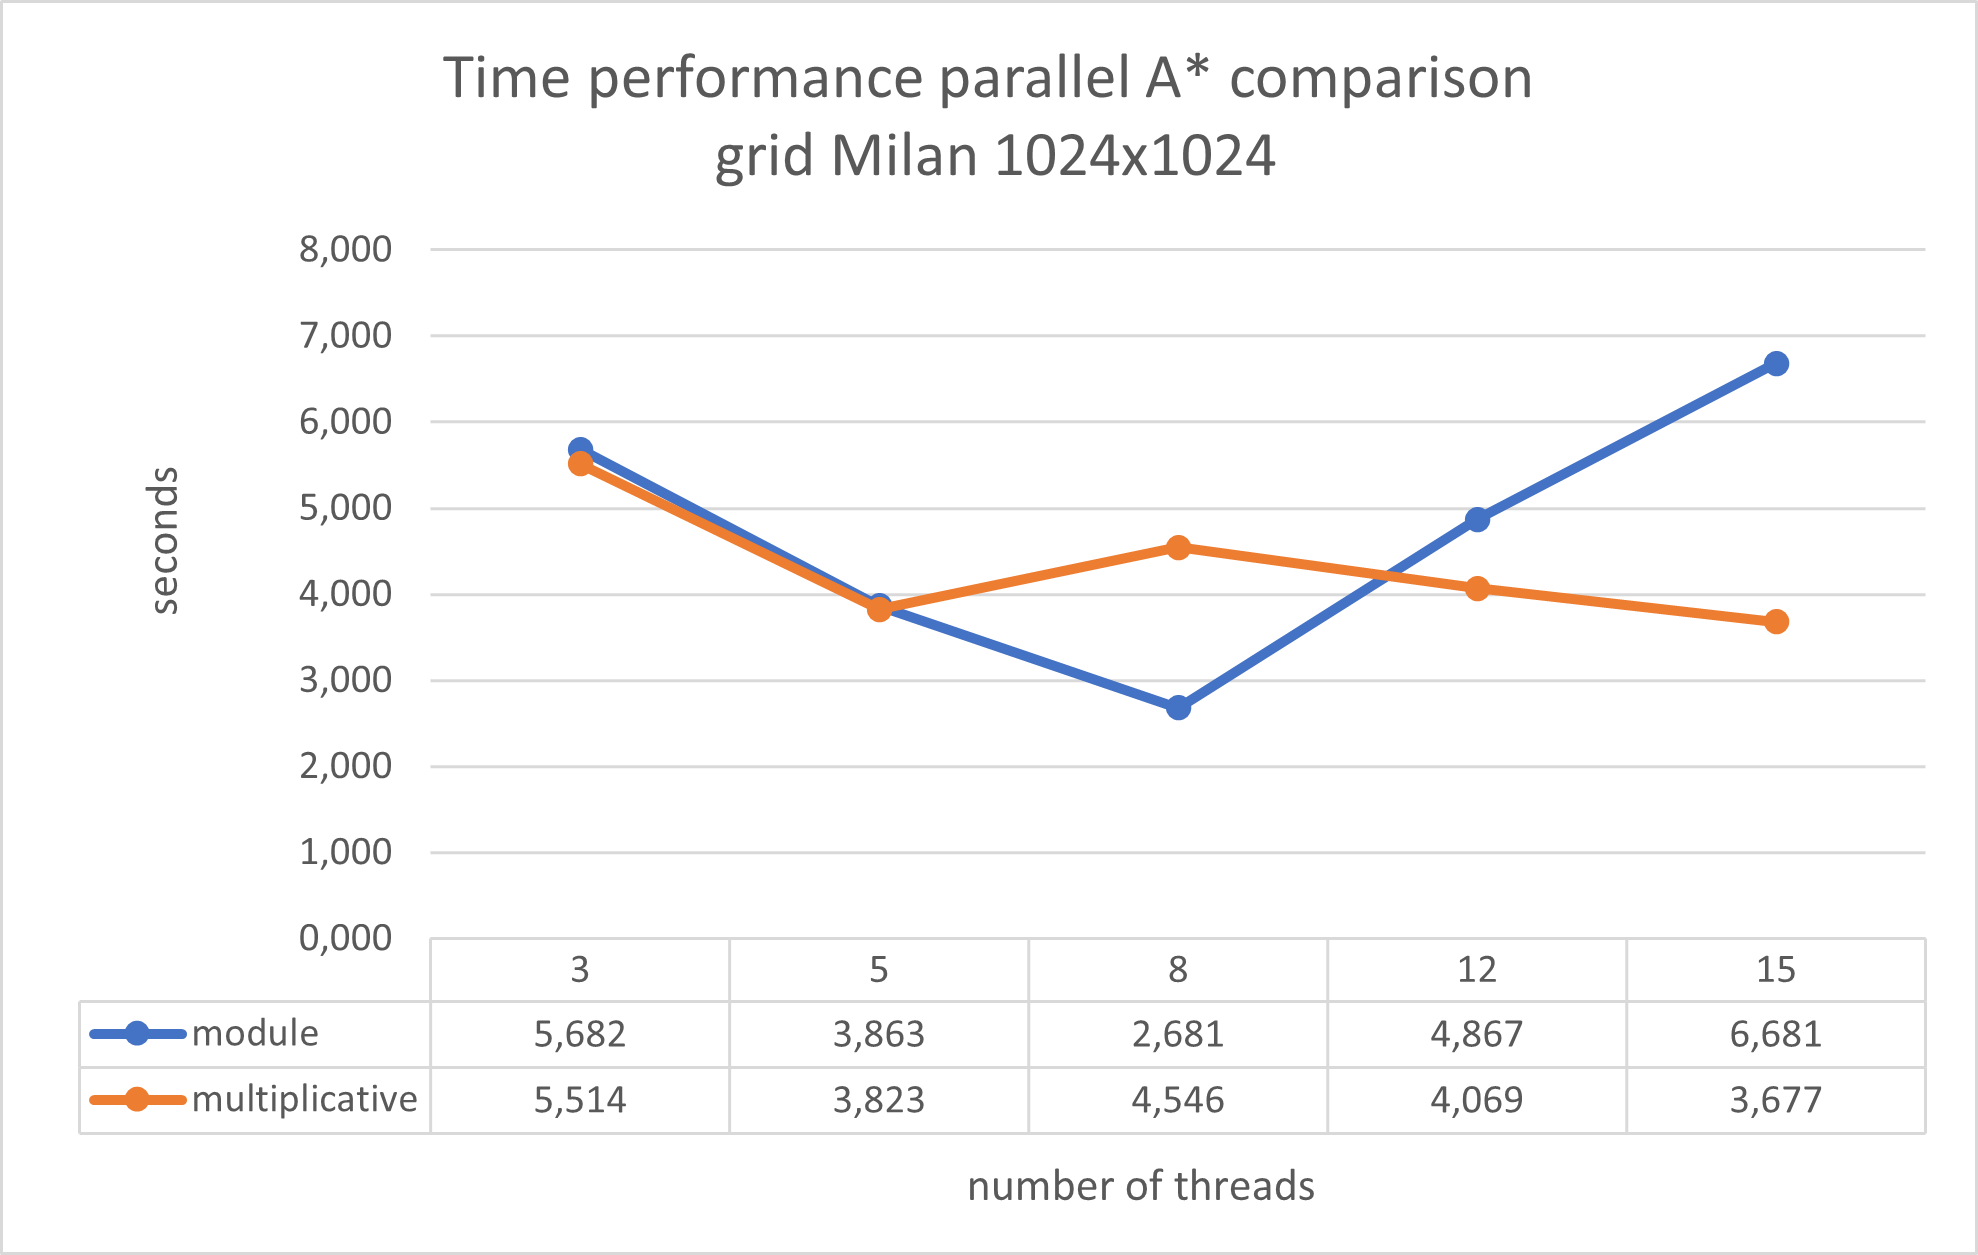
\includegraphics[scale=0.7]{milanParComparison.png}
    \caption{Performance comparison on different thread number and compute recipient function}
    \label{Milan par comp}
\end{figure}


Looking at the Figure \ref{Milan comp}, and considering that we choosed the best efficient number of threads for the parallel A*, 
we can notice a better performance compare to the sequential A* and the Dijkstra algorithms. 
To find the best result we tried the parallel A* changing the number of threads and the compute recipient function,
the Figure \ref{Milan par comp} shows all the experimental results of the tests.
Comparing the two compute recipient functions (simple module and multiplicative hash \ref{compute_reci})
on this relative small graph, the performance are comparable except on a big number of threads.


\subsubsection{Big Map}

To test more our algorithm we used a bigger graph, always with random weights, with about 4 Millions nodes.

\begin{figure}
    \centering
    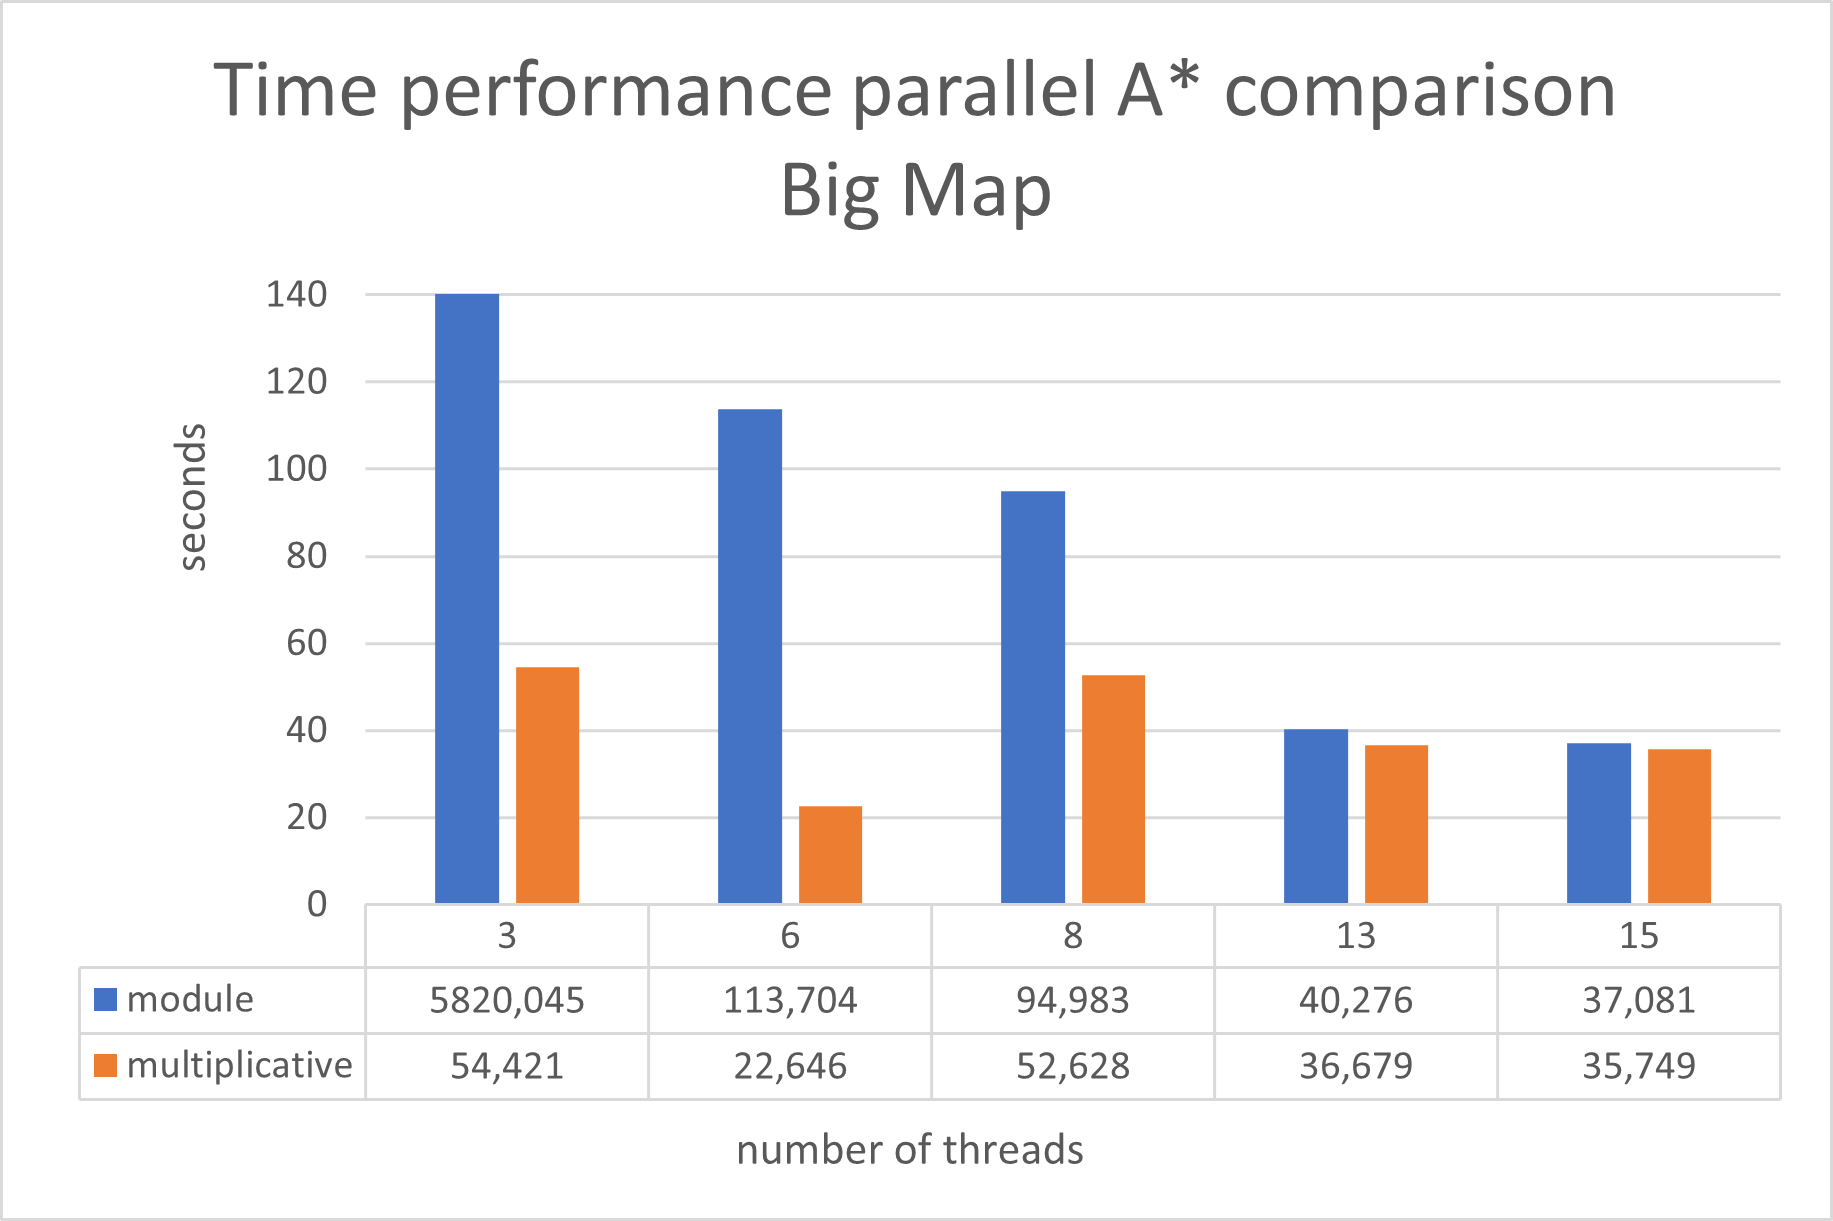
\includegraphics[scale=0.7]{mapParComparison.png}
    \caption{TODO}
\end{figure}






\subsection{memory occupation}
